\chapter{الأعداد العقدية} 


\section{مقدمة}
تنطلق دراسة التحليل العقدي من الحاجة الى  ايجاد حلول لمعادلات رياضية لا يوجد لها حل في الأعداد الحقيقية ، مثل المعادلة \(x^2 + 1 = 0\) حيث نلاحظ ان لو حاولنا حل هذه المعادلة بالطرق المعتادة
\begin{align*}
	x^2 + 1 = 0 ==> x^2 = -1 ==> x = \pm \sqrt{-1}
\end{align*}
نلاحظ إننا وصلنا الى جدار مسدود لأنه لا يوجد جذر تربيعي للأعداد السالبة ، ومن هنا تمت نشأة الأعداد العقدية حيث تم فرض $i = \sqrt{-1}$ أو $i^2=-1 $ أي أن المعادلة $x^2 + 1 = 0 $ يصبح لها حل وهو $\pm i$.

\section{تعريف الأعداد العقدية}
يعّرف العدد العقدي بالشكل 
\[
z = x + iy
\]
حيث \(x, y\) أعداد حقيقية و \(i^2 = -1\) ، ويسمى \(x\) بالجزء الحقيقي للعدد العقدي \(z\) ويرمز له بالرمز \(x = \re z\) و \(y\) بالجزء الخيالي أو التخيلي للعدد العقدي \(z\) ويرمز له \(y = \im z\).

\section{تمثيل الأعداد العقدية هندسياً}
كنا في الأعداد الحقيقية نستخدم خط الأعداد الحقيقية لتمثيل الأعداد الحقيقية على سبيل المثال الأعداد 
(\(-3, -\sqrt{2}, 1//2, e, 4\))
تتمثل بالشكل
\begin{center}
	\def\xscale{1}
	\def\yscale{1}
	\begin{tikzpicture}[x=\xscale cm, y=\yscale cm, thick]
		\draw[tri-tri] (-4, 0) -- (5, 0) node[below left, xshift=6pt] {};
		\foreach \x in {-3,-2,-1,0,1,2,3,4} {\draw[] (\x, 0.2/\yscale) -- (\x, -0.2/\yscale);}\foreach \x in {-3, -1.414, 1/2, 2.718, 4}{\fill[red] (\x, 0) circle (2.5pt);}
		\foreach \x in {-3,0,4} {
			\node[below=5pt] at (\x, 0) {$\x$};
		}
		\node[below=5pt] at (-1.414, 0) {$-\sqrt{2}$};
		\node[below=5pt] at (1/2, 0) {$\dfrac{1}{2}$};
		\node[below=5pt] at (2.718, 0) {$e$};
	\end{tikzpicture}
\end{center}
أما الأعداد العقدية تتمثل على مستوى الأعداد العقدية ثنائي الأبعاد ، لأنه العدد العقدي \(z = x + iy\) يتمثل بجزئين (الحقيقي و التخيلي) فالحقيقي يتمثل على الخط الأفقي والتخيلي يتمثل على الخط العمودي. أي أن 
\[
z = x + iy = (x, y)
\]
\begin{example}
	لنمثل الأعداد التالية
	\begin{tasks}[cols=3]
		\task \(z_1 = 1 + 2i\)
		\task \(z_2 = -3 - \sqrt{2} i\)
		\task \(z_3 = 4 - 4.2 i\)
		\task \(z_4 = -2 + 5//2 i\)
		\task \(z_5 = -3i\)
		\task \(z_6 = 3.5\)
	\end{tasks}
	
	\begin{center}
		\def\xscale{1}
		\def\yscale{1}
		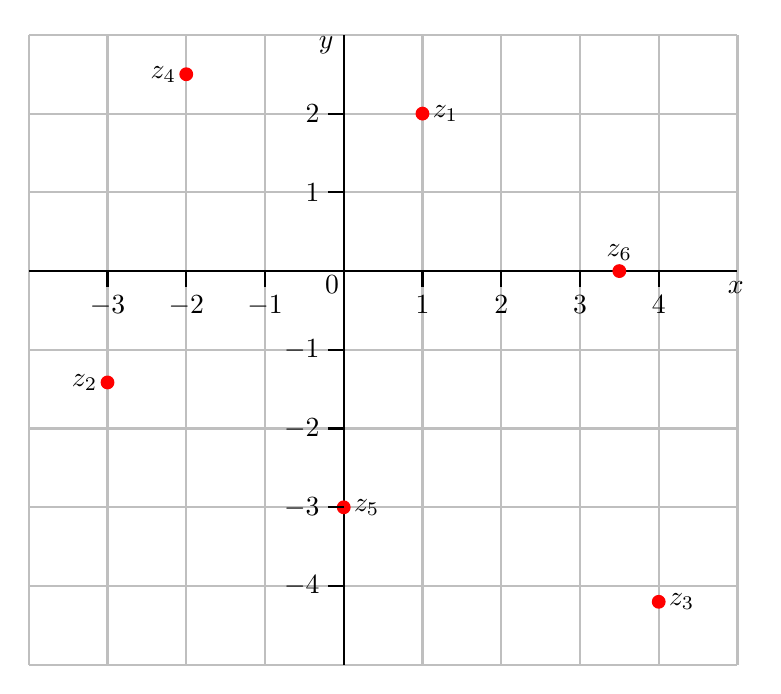
\begin{tikzpicture}[x=\xscale cm, y=\yscale cm, thick]
			\draw[gray!50] (-4, 3) grid (5, -5);
			\draw (-4, 0) -- (5, 0) node[below left, xshift=6pt] {$x$};
			\draw (0, -5) -- (0, 3) node[below left, yshift=3pt] {$y$};
			\node[below left, xshift=2, yshift=2] at (0, 0) {0} coordinate (O);
			
			\coordinate (z1) at (1,2);
			\coordinate (z2) at (-3, {-sqrt(2)});
			\coordinate (z3) at (4, -4.2);
			\coordinate (z4) at (-2, 5/2);
			\coordinate (z5) at (0, -3);
			\coordinate (z6) at (3.5, 0);
			
			
			
			
			\foreach \z in {z1, z2, z3, z4, z5, z6}{
				\fill[red] (\z) circle (2.5pt);
			}
			\foreach \x in {-3,...,-1,1,2,...,4} {\draw (\x, 0) -- (\x, -0.2/\yscale);}
			\foreach \x in {-3,...,-1,1,2,...,4} {
				\node[below=5pt] at (\x, 0) {$\x$};
			}
			
			\foreach \y in {-4,...,-1,1,2} {\draw (0, \y) -- (-0.2/\xscale, \y);}
			\foreach \y in {-4,...,-1,1,2} {
				\node[left=5pt] at (0, \y) {$\y$};
			}
			
			\node[right] at (z1) {$z_1$};
			\node[left] at (z2) {$z_2$};
			\node[right] at (z3) {$z_3$};
			\node[left] at (z4) {$z_4$};
			\node[right] at (z5) {$z_5$};
			\node[above] at (z6) {$z_6$};
		\end{tikzpicture}
	\end{center}
\end{example}

\section{العمليات على الأعداد العقدية}
مثل الأعداد الحقيقية سوف نتعرف على العمليات الاعتيادية الأربعة: الجمع ، الطرح ، الضرب والقسمة.\linebreak
ليكن \(z_1 = x_1 + iy_1 , \quad z_2 = x_2 + iy_2\)
\begin{tasks}[cols=1, label=\textbf{\arabic*.}, labelsep=5pt]
	\task \textbf{عملية الجمع:} تتم بجمع الجزء الحقيقي مع الحقيقي والتخيلي مع التخيلي
	\[
	z_1 + z_2 = (x_1 + x_2) + i(y_1 + y_2)
	\]
	
	\task \textbf{عملية الطرح:} كذلك تتم بطريقة مشابهة
	\[
	z_1 - z_2 = (x_1 - x_2) + i(y_1 - y_2)
	\]
	
	\task \textbf{عملية الضرب:} تتم من خلال عملية التوزيع الاعتيادي الذي تعلمناه من الأعداد الحقيقية 
	\begin{align*}
		z_1 z_2 &= (x_1 + iy_1) (x_2 + iy_2)\\
		&= x_1x_2 + ix_1 y_2 + i x_2 y_1 + i^2 y_1 y_2\\
		&= x_1x_2 + ix_1 y_2 + i x_2 y_1 - y_1 y_2\\
		&= (x_1x_2 - y_1y_2) + i (x_1y_2 + x_2 y_1)
	\end{align*}
	
	\task \textbf{عملية القسمة:} عندما نقسم \(z_1\) على \(z_2\) نضرب المقام (\(z_2 = x_2 + i y_2\)) بمرافقه \(x_2 - i y_2\)
	\begin{align*}
		z_1/z_2 &= (x_1 + iy_1)/(x_2 + i y_2) = (x_1 + iy_1)/(x_2 + i y_2) \cdot (x_2 - i y_2)/(x_2 - i y_2)\\
		&= (x_1x_2 + y_1y_2 + i (x_2y_1 - x_1y_2))/(x_2^2 + y_2^2) 
	\end{align*} 
\end{tasks}

\subsection*{خصائص العمليات على الأعداد العقدية}
\begin{tasks}[cols=1, label=\textbf{\arabic*.}, labelsep=5pt]
	\task \textbf{الإبدال:} عمليتي الجمع والضرب عمليتان ابداليتين
	\begin{tasks}[cols=2]
		\task \(z_1 + z_2 = z_2 + z_1\)
		\task \(z_1z_2 = z_2z_1\)
	\end{tasks}
	
	\task \textbf{التجميع:} خاصية التجميع تنطبق على الجمع والضرب
	\begin{tasks}[cols=2]
		\task \(z_1 + (z_2 + z_3) = (z_1 + z_2) + z_3\)
		\task \(z_1(z_2 z_3) = (z_1 z_2) z_3\)
	\end{tasks}
\end{tasks}

\begin{example}
	أوجد ما يلي وبسط الناتج الى الصورة القياسية للعدد العقدي
	\begin{tasks}[cols=2]
		\task \((1/(2-3i)) (1/(1+i))\)
		\task \((1+2i)/(3-4i) + (2-i)/5i\)
		\task \(5i/((1-i)(2-i)(3-i))\)
		\task \((1-i)^4\)
	\end{tasks}
\end{example}
\begin{solution}
	\begin{tasks}[cols=1]
		\task
		\[
		(1/(2-3i)) (1/(1+i)) = 1/(2 + 2i - 3i + 3) = 1/(5 - i) = 1/(5-i) \cdot (5 + i)/(5 + i) = (5 + i)/(25 + 1) = 5/26 + 1/26 i
		\]
		\task 
		\begin{align*}
				(1+2i)/(3-4i) + (2-i)/5i
				&= ((1 + 2i)(5i) + (2-i)(3 - 4i))/((3-4i)(5i))\\
				&= (5i - 10 + 6 - 8i - 3i - 4)/(15i + 20)\\
				&= (-8 - 6i)/(20 + 15i)\\
				&= (-2(4+3i))/(5(4 + 3i))\\
				&= -2/5
		\end{align*}
		بطريقة أخرى يمكننا حساب الناتج من خلال ايجاد قسمة كل كسر على حدى ومن ثم جمع الناتجين \HW.
		
		\task \HW
		
		\task 
		\(
		(1 - i)^4 = ((1-i)^2)^2 = (1 - 2i + i^2)^2 = (-2i)^2 = 4i^2 = -4
		\)
	\end{tasks}
\end{solution}

\section{القيمة المطلقة للعدد العقدي}
ليكن \(z = x + iy\) عدد عقدي، وكما تعلمنا سابقا ان العدد العقدي يتمثل كنقطة على المستوي العقدي (المستوي \(z\) أو المستوي \(xy\)) ، فأن القيمة المطلقة للعدد العقدي \(z\) تتمثل بطول قطعة المستقيم المرسومة من نقطة الأصل الى العدد العقدي نفسه ويرمز لها بالرمز \(|z|\)، كما في الشكل
\begin{center}
	\def\xscale{1}
	\def\yscale{1}
	\begin{tikzpicture}[x=\xscale cm, y=\yscale cm, thick]
		\draw (-1, 0) -- (5, 0) node[below left, xshift=6pt] {};
		\draw (0, -1) -- (0, 4) node[below left, yshift=3pt] {};
		\node[below left, xshift=2, yshift=2] at (0, 0) {$O$} coordinate (O);
		
		\coordinate (z) at (3.5, 2.5);
		\draw[color=gray, dashed] (z |- 0, 0) -- (z) --node[above]{$x$} (z -| 0, 0);
		\fill (z) circle (2.5pt);
		\draw[-tri, shorten >= 2pt, very thick] (O) --node[above, sloped]{$|z|$} (z);
		\node[right] at (z) {$z = x + iy$};
		\measureline{O}{3.5, 0}{$x$}{below}{-0.2}
		\measureline{3.5, 0}{3.5, 2.5}{$y$}{right}{-0.2}
		
	\end{tikzpicture}
\end{center}
نلاحظ تكوين مثلث قائم الزاوية ، أي يمكن ايجاد طول الوتر (القيمة المطلقة للعدد العقدي \(z\)) من خلال نظرية فيثاغورس
\[
|z|^2 = x^2 + y^2 => |z| = \sqrt{x^2 + y^2}
\]
